\section{Fejlesztői dokumentáció}
\subsection{Megoldási terv}
A rendszer több különálló modulból kell hogy álljon:
\begin{itemize}
\item Felhasználói weboldal, ahol a bejelentkezést végre akarják hajtani. Jelen esetben ez egy JavaEE backend (Spring Framework), és AngularJS frontendet használó alkalmazás. Ennek az alkalmazásnak a bejelentkezési mechanizmusa kell , hogy össze legyen integrálva az E-Group IDX szerverével. Erről az integrálásról a megvalósítás pontban írok részletesebben. Ez az oldal pusztán demonstrálásra lesz használva, egy publikus oldalról gesztikuláció alapú bejelentkezéssel egy védett oldalt lehet majd elérni, amely kiírja az azonosított felhasználó nevét. Kijelentkezés menüpont pedig bontja a munkamenetet.
\item Az E-Group IDX szervere, amelyben új modulként jelenik meg a gesztikuláció alapú bejelentkezés. Mivel a jelenlegi modulok hasonló, off-site kommunikációt egy kivételével nem tartalmaznak, így a jelenlegi limitáló tényezők miatt szükséges lesz egy authentikáló alkalmazásra is, amit az IDX szerver REST hívásokon keresztül el tud érni. A lényeges logika ebben a rendszerben kell megvalósuljon, ám a felhasználókról semmilyen adatot nem tartalmazhat permanensen.
\item Authentikáló alkalmazás, amely a belépési logikát tartalmazza. Egy IDX felületről indított bejelentkezésről REST-en keresztül üzenetet kell kapnia, majd ezt az rekordot társítani kell tudni egy a mobil alkalmazásból jövő üzenettel. A mobil alkalmazás üzenetei és az IDX szerverből érkező perzisztált rekord alapján valamilyen logika mentén a bejelentkezést el kell fogadnia vagy el kellutasítania. Ezt az üzenetet nem küldheti vissza az IDX szervernek, ehelyett user interakció vagy esetleges pollozó algoritmus kell lekérdezze tőle.
\item Android mobil alkalmazás, amely támogatja a regisztrációt és a bejelentkezést. Ez az alkalmazás az IDX vagy a felhasználói weboldal felületéről kell indítható legyen, innen megfelelő kezdeti paramétereketkell fogadnia, ami segítségével tudnia kell, hogy regisztráció illetve bejelentkezés esetén hova továbbítsa a feldolgozott adatokat. Az elektronikus személyi igazolvánnyal való kommunikációhoz a nyílt forráskódú JMRTD függvénytárat használjuk.
\item Egy vagy több third party arcfelismerő alkalmazás, amely hosszútávon lehet egy online, illetve offline megoldás is, beépítésekor törekedni kell a könnyű konfigurációra. Az authentikáló alkalmazás fogja hívni a bejelentkezés megfelelő lépéseiben, a válasz alapján lehet eldönteni a bejelentkezés sikerességét. Jelenleg a Microsoft Project Oxford és a Face++ kerül beépítésre
\end{itemize}

%Az alábbi ábra mutatja a rendszer komponenseit és azok kommunikációját. Az egyenes nyíl jelzi, ha az adott komponens meg tudja szólítani valamilyen módon a célkomponenst. A kérésre adott választ nem jelöltem.

%\begin{figure}[h]
% \begin{minipage}{1\textwidth} 
%\centering
  %  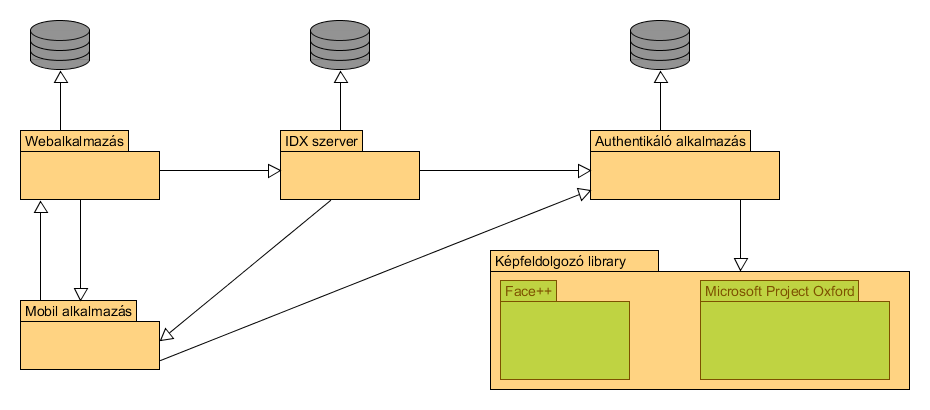
\includegraphics[scale=0.47]{img/rendszerkomponensek}
    %\caption{A rendszer komponensei}
 %\end{minipage}
%\end{figure}

\subsubsection{Felhasználó weboldal}
A publikus főoldalon van lehetőségünk bejelentkezni, illetve amennyiben még nincsen felhasználónk, regisztrálni. A bejelentkezés gombra kattintva megfelelő IDX integráció esetén az IDX bejelentkező felületére leszünk továbbítva. Regisztráció esetén egy felhasználónév megadásával indíthatunk új folyamatot. Itt ellenőrizni kell a felhasználónév szabad felhasználást, illetve mivel itt még csak paramétereket generálunk a mobilalkalmazásnak és a regisztrációs adatok csak később kerülnek adatbázisba, így ezt később is ellenőrizni kell! A regisztrációnál generálni kell egy olyan linket, amit a telefon megnyitva elindítja a mobilalkalmazást regisztrációs módban, és ennek a linknek tartalmaznia kell azokat a paramétereket ami alapján a megadott felhasználónévvel, a személyi igazolványból kiolvasott igazolványszámmal és igazolványképpel a regisztrációt véglegesíteni tudja a weboldalon.
Ezután egy új regisztrált felhasználónak kell megjelennie a mgfelelő táblában, és ezt a felhasználót regisztrálni kell az IDX szerver megfelelő táblájába is.
\\Az IDX integrációhoz szükséges táblákon kívül (ezeket a megvalósítás résznél írja le a fejezet), ez a modul egy adatbázis táblát tartalmaz.

\begin{figure}[h]
 \begin{minipage}{1\textwidth} 
\centering
    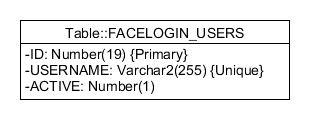
\includegraphics[scale=0.7]{img/facelogin_db}
    \caption{Felhasználó weboldal adatbázisszerkezet}
 \end{minipage}
\end{figure}


	\begin{tabular}{|p{4cm}|p{3cm} |p{4cm}|}
   	\hline
	\textbf{Mező neve} & \textbf{Érték} & \textbf{Szerep}\\ \hline
	ID & Number (19) & Szekvencia által generált érték, elsődleges kulcs \\ \hline
	USERNAME & VARCHAR(255 Byte) & Egyedi felhaszálónév  \\ \hline
	ACTIVE & Number (1) & Flag, ami jelzi, hogy a felhasználó aktív-e \\ \hline
	\end{tabular}

\subsubsection{IDX szerver}
A felhasználói weboldalhoz integrált IDX szerver felelős a beléptetés menedzseléséért, és a munkamenet tartásáért. Ez egy már kész szoftver, aminek egy új modulja a most elkészült gesztikuláció alapú bejelentkezés. A használatához több konfigurációs beállításra lesz szükségünk a későbbiekben kifejtett weboldal integráció során. A főbb részei az új modul fejlesztésének: 
\begin{itemize}
\item Jelenjen meg az eddigi modulok között egy új lehetőségként
\item Amennyiben ezt az új modult használjuk bejelentkezéshez, saját képernyői legyenek, és saját táblából töltse be a felhasználóit
\item Minden más munkamenet kezeléshez integrálódjunk, ezt a már meglévő rendszer ugyanis tudja menedzselni. Mi csak a felhasználó betöltést végezzük saját logika alapján
\item A saját logika delegálja a feladatokat az authentikáló alkalmazásnak REST hívásokon keresztül. Adjon át minden olyan adatot, amely az azonosításhoz szükséges. Ilyenek a felhasználónév, a bejelentkezési kérelemhez generált id, az elmentett személyi igazolvány képe, személyi igazolvány száma és a kért kihívás azonosítója.
\item Azokat a paramétereket (generált id és az authentikáló alkalmazás eléréséhez szükséges URL) amik szükségesek a mobil alkalmazás bejelentkezést végrehajtó műveleteihez, egy linken a feületre kell generálni, ami elindítja a mobil alkalmazást bejelentkezés módban
\item A bejelentkezési kérelem delegálása után pollozással vagy felhasználói interakcióval REST híváson keresztülellenőrizze, hogy az adott generált id-hoz tartalmazó kérelem megerőítésre került-e
\item Sikeres megerősítés után delegáljuk a bejelentkezés további lépéseinek végrehajtását a már meglévő modulokhoz.
\end{itemize}

\begin{figure}[h]
 \begin{minipage}{1\textwidth} 
\centering
    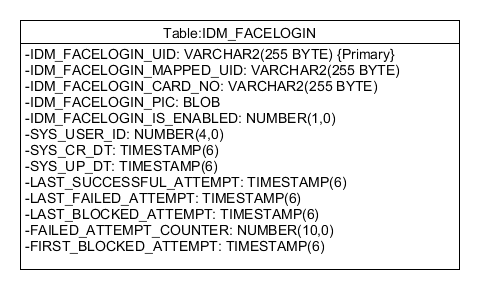
\includegraphics[scale=0.7]{img/facelogin_idm_db}
    \caption{IDX szerver user adatbázistábla}
 \end{minipage}
\end{figure}

Fontosabb mezők leírása:

\begin{tabular}{|p{6.5cm}|p{3cm} |p{4cm}|}
   	\hline
	\textbf{Mező neve} & \textbf{Érték} & \textbf{Szerep}\\ \hline
	IDM\_FACELOGIN\_UID & VARCHAR2(255 BYTE) & Felhasználónév, elsődleges kulcs \\ \hline
	IDM\_FACELOGIN\_MAPPED\_UID & VARCHAR2(255 BYTE) & Felhasználónév. Más modulok esetén nem feltétlen ugyanaz mint az előző mező, de itt minden esetben megegyezik \\ \hline
	IDM\_FACELOGIN\_CARD\_NO & VARCHAR2(255 BYTE)& Személyi igazolvány száma \\ \hline
	IDM\_FACELOGIN\_PIC & BLOB & Bináris formában mentett igazolványkép \\ \hline
	IDM\_FACELOGIN\_IS\_ENABLED & NUMBER(1,0) & Flag, ami jelzi, hogy a felhasználó aktív-e \\ \hline
	\end{tabular}


Ez a modul két képernyő megjelenítését kívánja meg. Első amikor a felhasználó begépeli a bejelentkeztetni kívánt felhasználónevet. Ezt a rendszer ellenőrzi, és ha létezik és aktív, megjeleníti a következő képernyőt. Ezen a felületen két lehetősége van a felhasználónak: megnyitja a mobil applikációt vagy a bejelentkezsére kattint. Hibás bejelentkezési kérelem esetén (a bejelentkezési kérelem nem lett még mobiltelefonon keresztül megerősítve), a kérelem elutasításra kerül, és visszairányításra kerül a felhasználó a kiinduló weboldalára.

\subsubsection{Mobil alkalmazás}
A mobil alkalmazás egy android rendszeren futó segégszoftver a bejelentkezés szükséges lépéseinek végrehajtásához. Két üzemmódja létezik:
\begin{itemize}
\item Regisztráció
\item Bejelentkezés
\end{itemize}

Mindkét üzemmód használatának előfeltétele a kártyaadatok helyes megadása, az alkalmazás erre előkészített felületéről való indítása (a szükséges paraméterek megléte nélül nem használható) és az NFC bekapcsolása. Ezeknek a feltételeknek hiányosságairól az alkalmazás indításkor figyelmeztet. Javítás után a felhasználó folytathatja a megkezdett folyamatot. Következő lépés az elektronikus személy hátlaphoz tartása. A kártya olvasásában a nyílt forráskódú JMRTD lesz segítségünkre, amely először egy BAC (Basic Access Control) authentikációt hajt végre a megadott kártyaadatokkal (kártyaszám, születési dátum, lejárat dátuma), majd sikeres authentikáció esetén lehetőségünk nyílik a kártya szükséges adatainak olvasására.
\\Regisztráció esetén a kártyaszámot és az igazolványképet kell kiolvasni és visszaküldeni a felhasználói weboldalra az inicializáláskor megkapott link segítségével.
Bejelentkezés esetén először a kártyaszámot kell kiolvasni, és a szintén inicializáláskor megkapott paraméterekkel az authentikáló alkalmazásnak továbbítani. Amennyiben az alkalmazás ezt elfogadja, sikeres választ kapunk, különben hibaüzenetet, amit megjelenítünk a képernyőn. Sikeres válasz esetén a válaszban kell szerepeljen a kért kihívás. Új felületen az előlapi kamera képét kell megjeleníteni, majd gombnyomásra indítani a kihívást. Célszerű pár másodperc visszaszámlálást beépíteni, hogy a felhasználó az ilyenkor megjelenő kihívás szövegére gyorsan fel tudjunk készülni. Ezután felvesszük a választ, transzformációkat hajtunk végre (elfordítás 90 fokkal, tükrözés), tömörítünk, és kiválasztunk egyenlő időközönként maximum N darab képkockát, majd továbbítjuk az authentikáló alkalmazásnak párhuzamosan a bejelentkezési kérelem generált azonosítójával együtt, hogy a szerver tudja csatolni a megfelelő rekordhoz. Az erre kapott választ pedg feldolgozzuk és kiírjuk a felületre. Sikeres és sikertelen bejelentkezés esetén is gombnyomásra bezárjuk az alkalmazást, és visszatérünk az IDX felületére.

\subsubsection{Authentikáló alkalmazás}
Ennek a modulnak a célja, hogy minden felhasználói adat permanens tárolása nélkül egy bejelentkezési kérést elfogadjon vagy elutasítson. Fogadnia kell tudni az IDX felületéről REST híváson keresztül indított bejelentkezási kérelmet, ezt adatbázisba tárolni kell. Miután a megadott bejelentkezési időtartam lejárt, egy automata műveletnek ezt a régi, már nem használható bejegyzést törölnie kell.\\
Fogadnia kell továbbá három különböző kérést REST-en keresztül a mobil alkalmazásból:
\begin{itemize}
\item Személyi igazolvány szám és generált bejelentkezési azonosító fogadása a bejelentkezés első lépésének ellenőrzésére. Ha talál olyan rekordot a megerősítésre váró kérések táblájában amely az adott azonosítóhoz ugyanezt az igazolványszámot rendeli, és még a maximum időtartamon belül van, úgy ezt a lépést el kell fogadni, és válaszüzenetben a mobilalkalmazásnak vissza kell küldenie a rekordhoz tartozó kihívás szöveges leiratát. Hiba esetén a válasz törzsében a hiba okát meg kell jegyezni, ezt később a mobil alkalmazás feltudja dolgozni.
\item Kihíváshoz tartozó kékockákat kell fogadnia. Ezeket a mobil kliens párhuzamosan küldi a hozzájuk tartozó generált azonosítóval, azonosítónként pedig csoportosítani kell a beérkezett képeket. Érdemes a gyorsaság szempontjából nem adatbázisban, hanem memóriában tárolni ezeket, de ez esetben fontos a törlésükről nem megfeledkezni!
\item Miután a mobil alkalmazás minden képet felküldött, egy "nyugtát" küld, hogy minden adat megérkezett, és azt a nyugtát fogadva a kihívásra adott válasz kiértékelését el kell kezdeni. A kiértékelés eredményéről pedig a nyugtára adott válaszüzenetben tájékoztatni kell a mobil kilenst.
\end{itemize}

\begin{figure}[h]
 \begin{minipage}{1\textwidth} 
\centering
    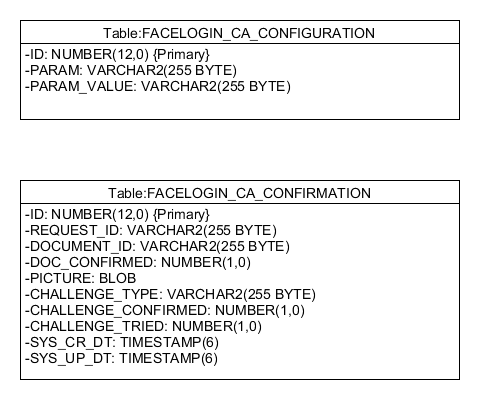
\includegraphics[scale=0.4]{img/facelogin_ca_db}
    \caption{Authentikáló alkalmazás táblái}
 \end{minipage}
\end{figure}
%\newpage
Mezők leírása:

\begin{tabular}{|p{5.5cm}|p{3cm} |p{6cm}|}
   	\hline
	\textbf{Mező neve} & \textbf{Érték} & \textbf{Szerep}\\ \hline
	ID & NUMBER(12,0) & Generált azonosító, elsődleges kulcs \\ \hline
	REQUEST\_ID & VARCHAR2(255 BYTE) & Az IDX szerverből kapott generált azonosító. A mobil alkalmazásból kapott adatokat is ezzel tudjuk majd azonosítani \\ \hline
	DOCUMENT\_ID & VARCHAR2(255 BYTE)& Személyi igazolvány száma \\ \hline
	DOC\_CONFIRMED & NUMBER(1,0) & Személyi igazolvány mobilos megerősítése után vátozik igazzá\\ \hline
	PICTURE & BLOB & IDX modulból kapott, bináris formában mentett igazolványkép\\ \hline
	CHALLENGE\_TYPE & VARCHAR2(255 BYTE)& A kért kihívás azonosítója, a rendszerben egy Enum értéknek felel majd meg. Ez az Enum fogja tartalmazni a kihívás szöveges leírását \\ \hline
	CHALLENGE\_CONFIRMED & NUMBER(1,0)& A kihívás elfogadása után válik igazzá \\ \hline
	CHALLENGE\_TRIED & NUMBER(1,0) & Amenyiben a kihívást már megpróbáltuk teljesíteni, igazzá válik. Az időlimiten belüli újrapróbálkozások ellen véd \\ \hline
	SYS\_CR\_DT & TIMESTAMP(6)& A bejelentkezési kérelem regisztrálásának időpontja \\ \hline
	SYS\_UP\_DT & TIMESTAMP(6)& Rekord frissítésének időpontja \\ \hline
\end{tabular}


%\begin{sidewaysfigure}
%\centering

   %      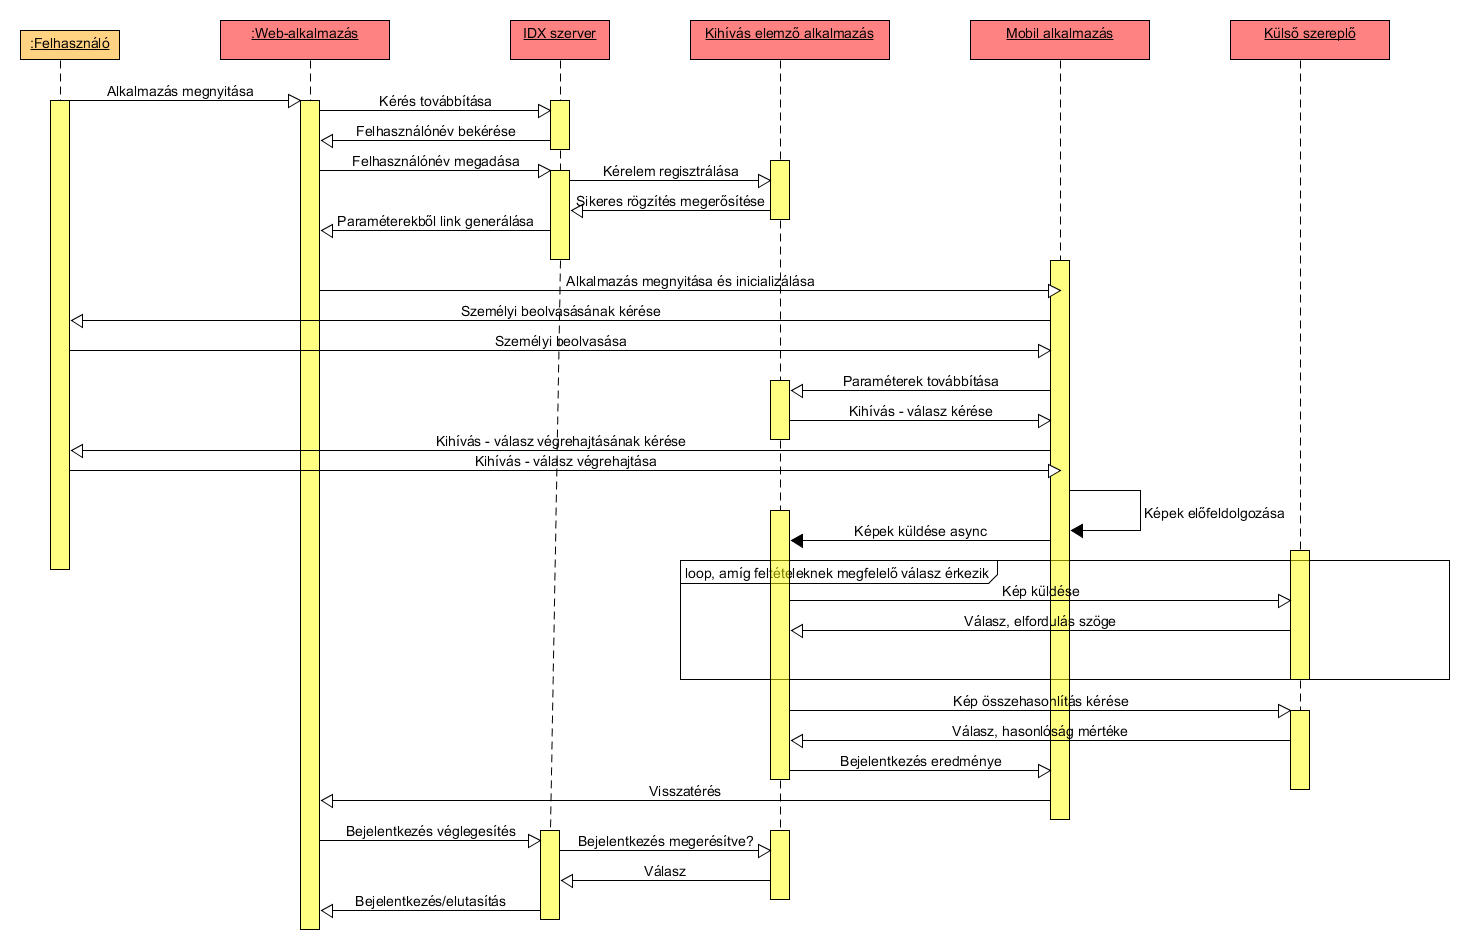
\includegraphics[scale=0.47]{img/szekvencia}

    %\caption{Bejelentkezés szekvencia diagramja}
%\end{sidewaysfigure}